\section{Memoria del proyecto}
\label{memoria}
\emph{En este capítulo se describirá cómo se ha llevado a cabo el proyecto, qué cambios se han hecho respecto a la versión inicial, imprevistos surgidos, etc}

A continuación se describen los objetivos principales de cada uno de los equipos de trabajo así como un pequeño resumen de cómo se ha desarrollado el trabajo de cada equipo en esta primera iteración. En el resto de la sección se describe detalladamente todo el desarrollo del proyecto.\\

\subsubsection*{FrontEnd y Middleware}
El principal objetivo del Frontend eran desarrollar las interfaces con las que los usuarios interaccionarían con la aplicación. Se distinguen dos interfaces, las de navegación web y la parte jugable del guiñote. La parte jugable se ha podido implementar en su mayoría, a falta del modo espectador y la parte de personalización. Sin embargo, la parte de la interfaz de navegación se completará para la segunda iteración, ya que únicamente se tienen las pantallas de login y la navegación.
\\
En cuanto al Middleware, el principal objetivo era comunicar la interfaz de juego para que los usuarios puedan jugar entre ellos, que se ha conseguido con éxito. Aun así, es necesario completar con la funcionalidad de que un usuario puede cambiar de dispositivo en una misma partida.

\subsubsection*{BackEnd}
El objetivo del equipo backend era desarrollar un paquete de java que representase la lógica del juego del guiñote, al mismo tiempo que desarrollaba gran parte de la página web dinámica del proyecto. Sin embargo, a mitad de desarrollo el trabajo, se centró en acabar la parte de la lógica del juego. Dicho objetivo se ha cumplido completamente con algunos retrasos en la entrega. Como consecuencia la web dinámica arrastra un leve retraso que deberá ser compensado en la segunda iteración. A pesar de dichas dificultades el equipo ha trabajado mucho para conseguir una primera versión funcional antes de la primera iteración.

\subsubsection*{Base de datos}
Los dos principales objetivos del equipo de bases de datos eran por una parte diseñar e implementar la base de datos para el sistema(esquema conceptual, lógico y físico) y por otra desarrollar la capa de acceso a datos proporcionando una interfaz para el backend. Los dos objetivos se han cumplido prácticamente en su totalidad, con excepción de la parte de acceso a datos relacionada con los torneos, que no ha sido posible terminar de implementar y será finalizada en la segunda iteración. Exceptuando las pequeñas dificultades iniciales relacionadas con un tardío diseño de la interfaz de acceso a datos, tanto la comunicación entre los miembros del equipo como con el resto de equipos relacionados con el acceso a los datos se ha desarrollado sin problemas.

Como decisión importante, destaca que tras un análisis del progreso del proyecto y adecuación a la planificación, el equipo de Bases de Datos iba más avanzado y tenía mucha menos carga de trabajo de cara a la segunda iteración que los equipos de BackEnd y FrontEnd. Por ello, antes de que los miembros del BackEnd comenzaran a trabajar en la Inteligencia Artificial (como así estaba decidido en un principio) se decidió reconfigurar el equipo de Inteligencia Artificial y que pasaran a formar parte de él los miembros del de Bases de Datos, con una organización final como la que se muestra en el organigrama de la sección \ref{organiz}.

\subsection{Inicio del proyecto}
\label{Inicio del proyecto}
\emph{Describir cómo transcurrió esta fase del proyecto, especialmente los resultados de llevar a cabo los procesos descritos en la sección Procesos de inicio del proyecto.}
\subsubsection*{FrontEnd y Middleware}
Dado que ningún integrante de este equipo de trabajo poseía conocimientos acerca de las tecnologías utilizadas (Phaser, JavaScript y WebSockets), se han formado mediante tutoriales gratuitos ofrecidos en diferentes páginas.
Para aprender los conocimientos fundamentales de Phaser, se realizaron ejemplos de pequeños juegos disponibles en la página Web oficial de los desarrolladores. Como Phaser utiliza fundamentalmente JavaScript, éste se ha aprendido de forma simultánea. Una vez se conoce la estructura de un juego, se comienza a desarrollar una parte de la interfaz y el esqueleto de las mismas. Cuando no se tenía claro como hacer determinada función, se accedían a los ejemplos disponibles en la web oficial de Phaser.

Para el aprendizaje de WebSockets, se han buscado ejemplos en Internet hasta dar con uno que resuelve el principal problema del proyecto: conseguir comunicación síncrona entre JavaScript y un back-end implementado en Java. El ejemplo se estudió y se analizó para adaptarlo a la necesidad.


\subsubsection*{BackEnd}
Durante la primera semana el equipo adquirió y configuró el software de desarrollo intellij IDEA. Como el proyecto necesitaba realizar pruebas con JUnit y desarrollar en entornos java y web dinámicas se necesita un proyecto JavaEE. Estas caracteristicas requieren la versión Ultimate de pago. Se ha utilizado la cuenta gratuita de estudiante proporcionada por la Universidad de Zaragoza, ya que la versión Community no ofrece estas funcionalidades.
Tras una primera toma de contacto comenzaron dos semanas de trabajo. Sin embargo, a lo largo de la primera iteración el equipo se ha encontrado con diferentes problemas de integración debido a la falta de experiencia del IDE. Por lo tanto en futuros proyectos sería recomendable incluir en formación horas para el aprendizaje de los IDE's.

\subsubsection*{Base de datos}
En el inicio del proyecto el equipo realizó la configuración de la base de datos en AWS, utilizando Amazon Aurora sobre MySQL como se había decidido. Las principales características de la base de datos utilizada para el proyecto se detallan a continuación:

\begin{itemize}
	\item Versión Software: Aurora MySQL 5.7.12
	\item Hardware: 1 CPU, 2GB RAM
	\item Identificador de la Intancia: sotayrey-aurora
	\item Identificador del Cluster: sotayrey-cluster
	\item Identificador de la base de datos: sotayrey\_db
	\item Copia de Seguridad: Cada 30 días
\end{itemize}

Las características seleccionadas se deben al requerimiento de utilizar solamente aquellos recursos disponibles para la versión gratuita de estudiantes, que es con la que se está trabajando. Además, el servidor de base de datos se ha configurado de forma que se puede acceder desde el exterior para hacer más fácil el acceso durante el desarrollo de la base de datos, pero este será deshabilitado una vez el sistema esté desplegado, por razones de seguridad.\\

En cuanto a formación, el equipo de bases de datos se formó en el funcionamiento de la api JDBC, así como en la utilización de pools de conexiones con c3p0. Al contrario de lo que se había establecido en los procesos de inicio del proyecto (sección \ref{inicio}), el equipo no se formó en lo que respecta a HTML/CSS y JSP, porque no lo requería para sus competencias en la primera iteración.
\subsection{Ejecución y control del proyecto}
\label{Ejecucion y control del proyecto}
Los procesos de control no se han llevado a cabo tal y como estipulaba el primer plan de gestión. Ya que el director del proyecto no se ha coordinado con los responsables de grupo. Sin embargo a nivel local, los responsables de grupo si han dirigido y organizado sus respectivos grupos. Además no se ha producido ninguna situación que requiera de mediación ni necesidad de intervención extraordinaria por parte de los responsables. 
Los procesos técnicos se han llevado a cabo tal y como estaban especificados en la primera versión del plan de gestión. Tanto en el apartado de pruebas como documentación. Aplicar los procesos acordados ha costado bastante por la falta de costumbre, sin embargo los ficheros fuente, pruebas y documentación obtenidos nos han permitido trabajar de forma más eficiente.
\subsubsection{Reparto del trabajo}
En un primer momento, el reparto de trabajo fue definido únicamente en relación a los equipos creados, como se detalla en la sección \ref{repartotrabajo}. Sin embargo, se detectó que este reparto, aunque necesario, era demasiado genérico y no permitía medir el progreso de forma clara. Por ello se decidió que dentro de cada equipo de trabajo se llevaría a cabo una división del trabajo en tareas o paquetes de trabajo, siguiendo la Estructura de Descomposición del Trabajo (WBS \cite{edt}). Cada paquete de trabajo corresponde a una tarea específica y claramente delimitada, como puede ser el desarrollo de una clase, y especifica un único responsable de este (no significa que sea la única persona que trabaje en él pero sí la responsable de su desarrollo). Para el control del progreso en relación a esta división del trabajo se ha utilizado el apartado Projects de GitHub, en el que cada paquete se marca con un tick cuando está finalizado y depurado.

A continuación se muestran los diagramas de paquetes desarrollados:

\begin{figure}[H]
		\hspace{-2cm}
		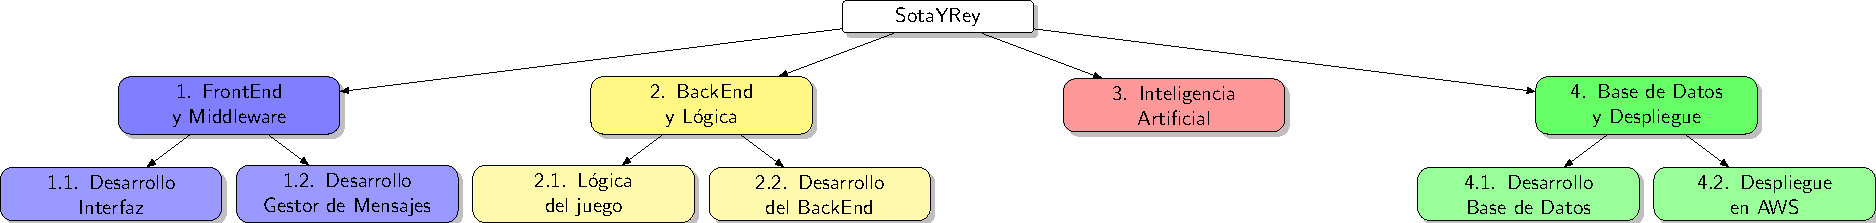
\includegraphics[scale=0.6]{figuras/edtGeneral.pdf}
		\caption{Diagrama general de reparto del trabajo}
	\end{figure}

\begin{figure}[H]
		\centering
		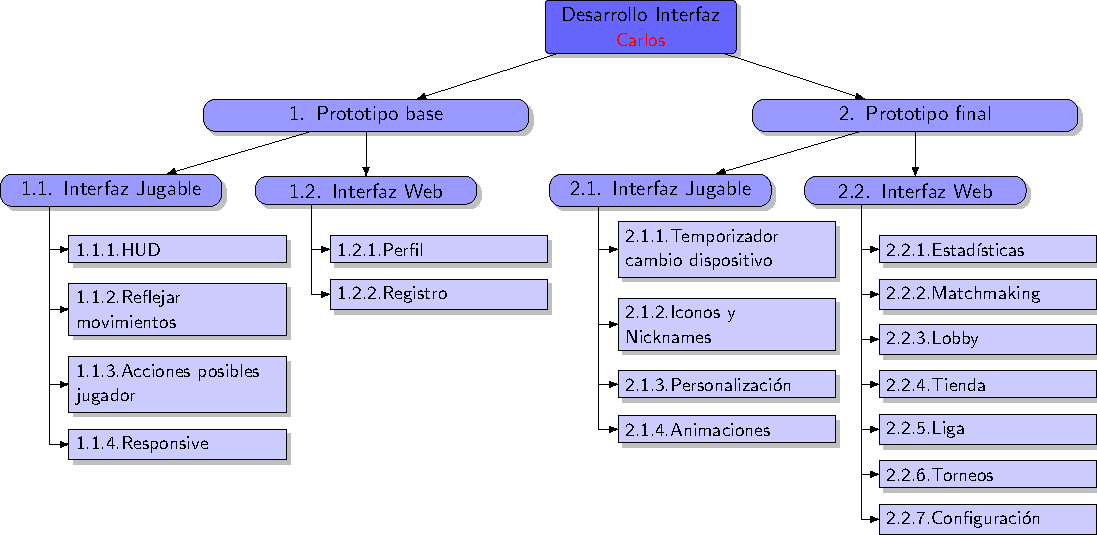
\includegraphics[scale=0.85]{figuras/edtInterfaz.pdf}
		\caption{Diagrama de Paquetes de Trabajo Interfaz}
	\end{figure}

\begin{figure}[H]
		\hspace{-2cm}
		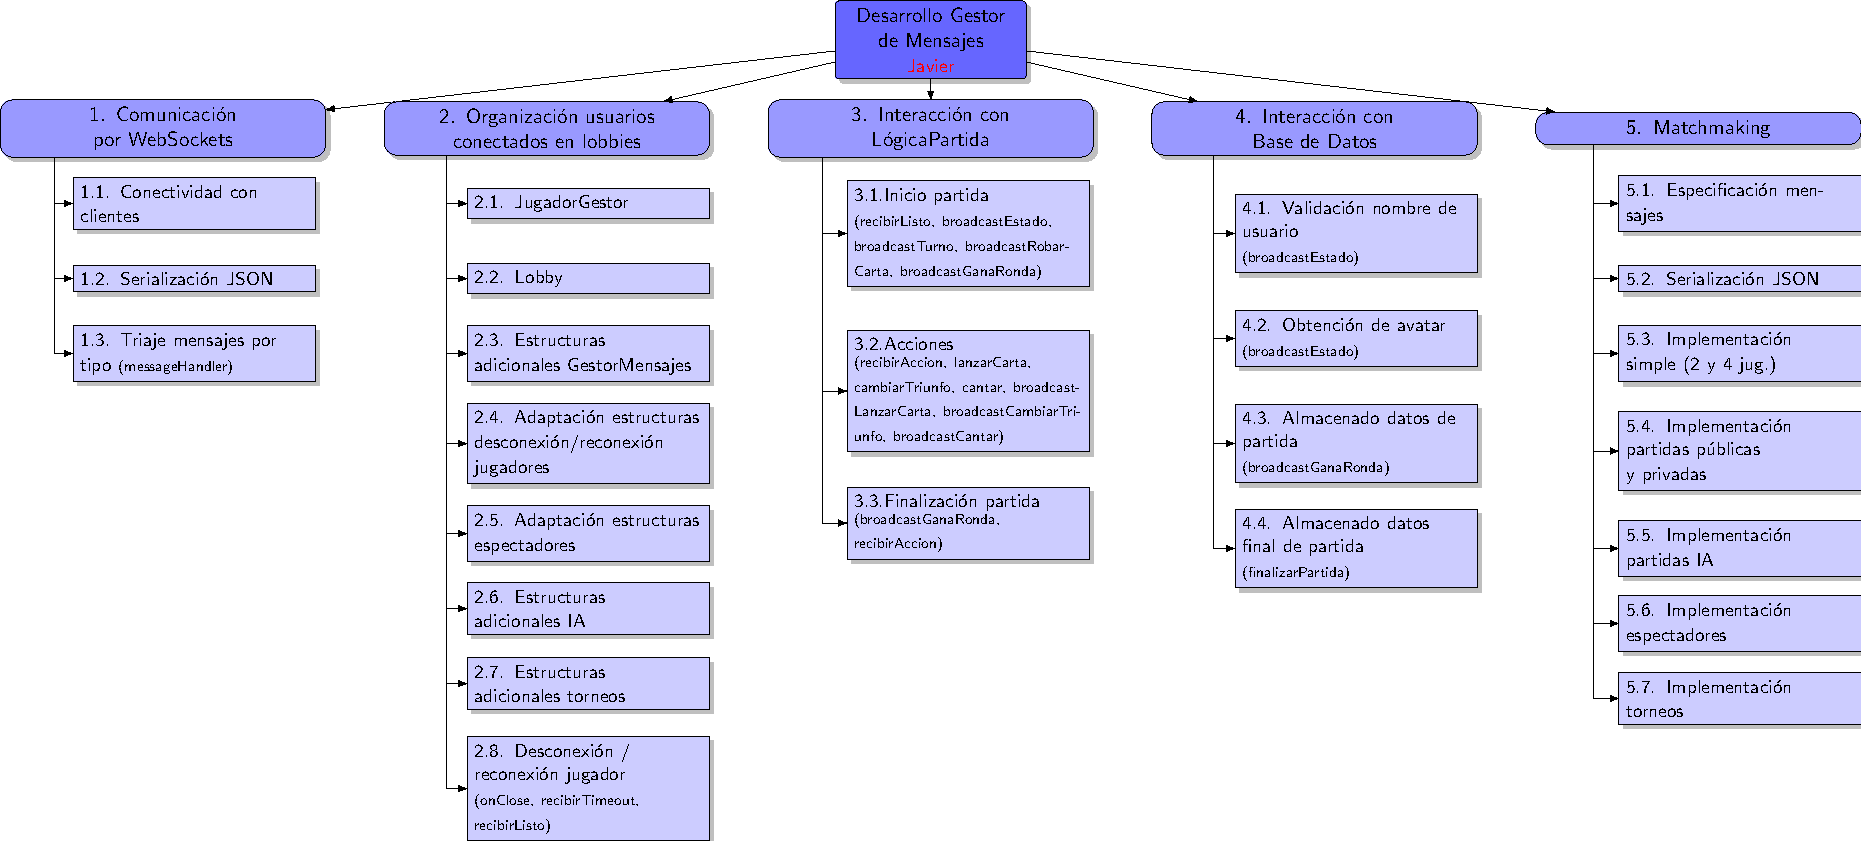
\includegraphics[scale=0.75]{figuras/edtGestorMensajes.pdf}
		\caption{Diagrama de Paquetes de Trabajo Gestor de Mensajes}
	\end{figure}


\begin{figure}[H]
		\centering
		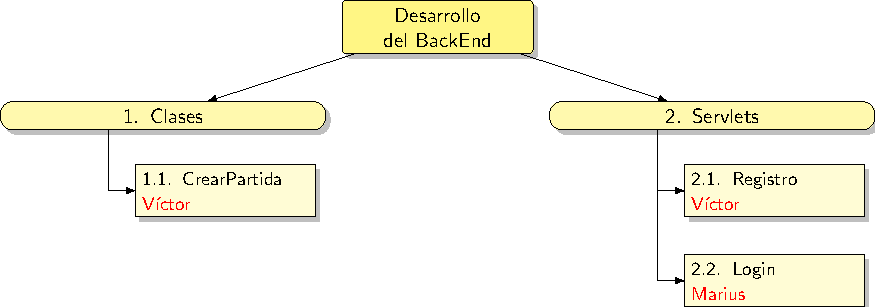
\includegraphics[scale=0.8]{figuras/edtBackend.pdf}
		\caption{Diagrama de Paquetes de Trabajo BackEnd}
	\end{figure}

\begin{figure}[H]
		\hspace{-1cm}
		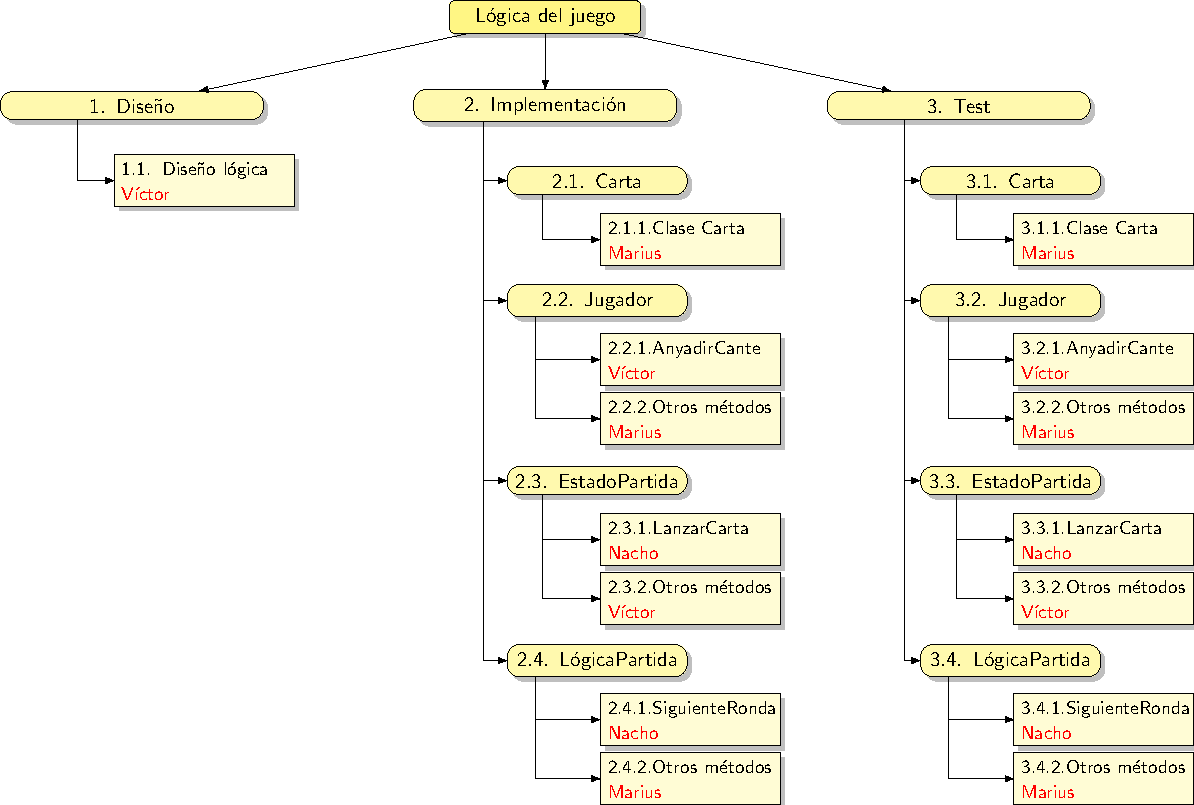
\includegraphics[scale=0.8]{figuras/edtLogica.pdf}
		\caption{Diagrama de Paquetes de Trabajo Lógica}
	\end{figure}

\begin{figure}[H]
		\hspace{-2cm}
		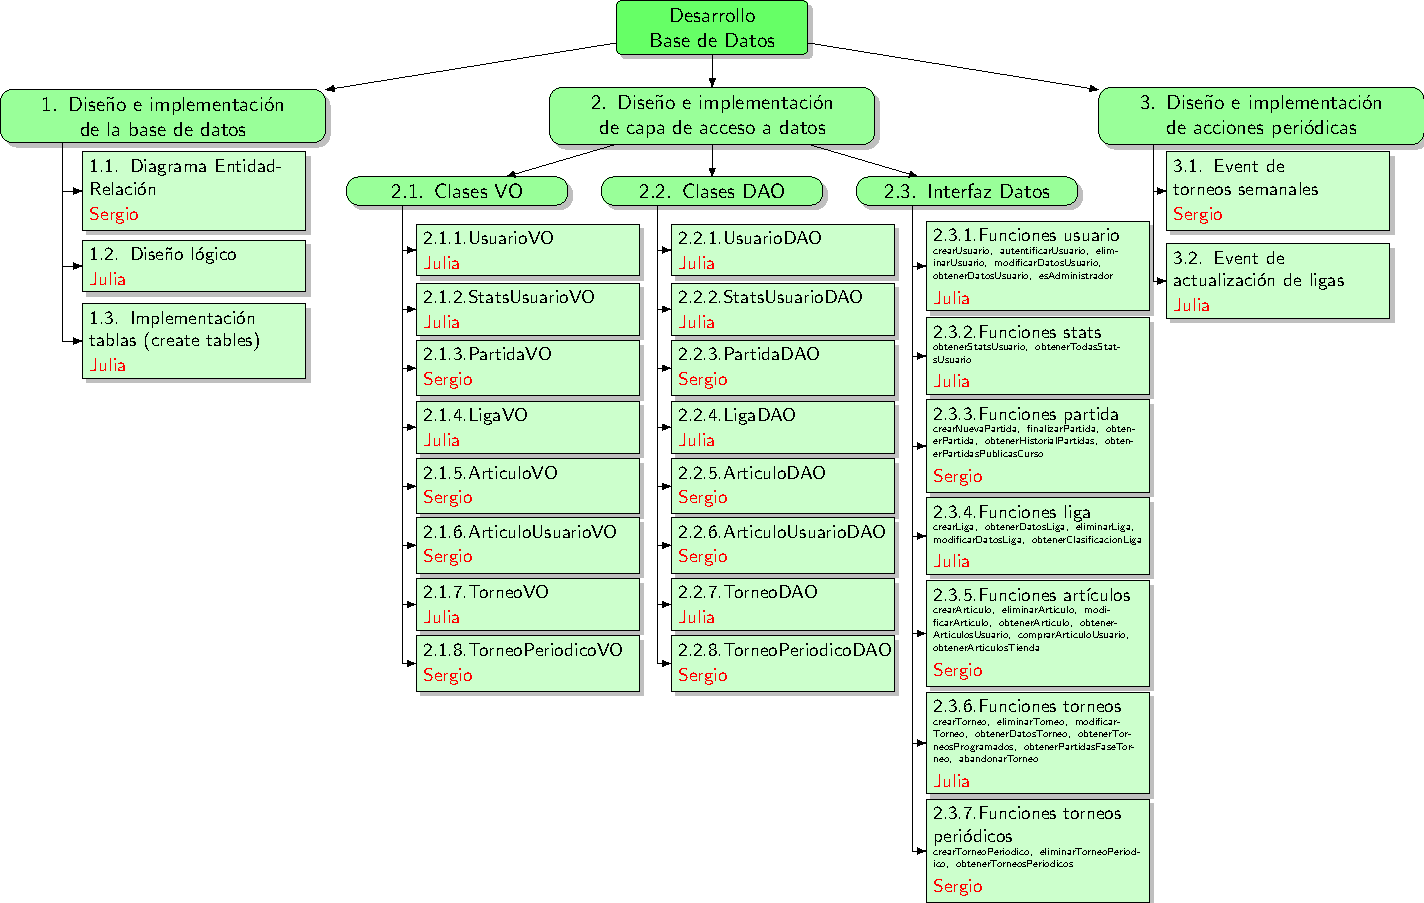
\includegraphics[scale=0.8]{figuras/edtBasesDatos.pdf}
		\caption{Diagrama de Paquetes de Trabajo Bases de Datos}
	\end{figure}

\begin{figure}[H]
		\centering
		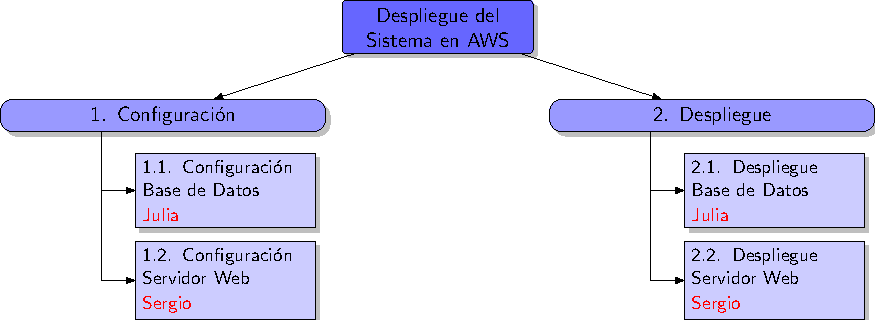
\includegraphics[scale=0.8]{figuras/edtDespliegue.pdf}
		\caption{Diagrama de Paquetes de Trabajo Despliegue}
	\end{figure}

Es importante añadir que el trabajo de integración de los diferentes paquetes de trabajo no está reflejado en estos diagramas pero también ha sido necesario repartirlo y realizarlo. A su vez, algunos de los paquetes correspondientes a la segunda iteración no se han diseñado todavía, o aunque se haya hecho, podrían producirse modificaciones sobre ellos ya que todavía no se han analizado ciertas partes a fondo.
\subsubsection{Comunicación interna}
La decisión de la nueva estructura de grupos se realizó mediante una reunión entre los miembros afectados por el cambio.
En cuanto a la parte de BackEnd, al comienzo del proyecto la comunicación ha sido bastante pobre, ya que en algunos momentos los desarrolladores han realizado la misma actividad por duplicado. En el desarrollo de los diferentes componentes cada miembro tenía su propio diseño en mente y ha sido necesario ponerse de acuerdo y plasmar el diseño en un diagrama UML de clases, que todos pudieran consultar y hacer referencia. Hacia el final de la primera iteración el equipo ha mejorado su comunicación en gran medida.
\\
La comunicación entre los diferentes equipos se ha llevado a través del servicio de terceros Skype para, principalmente, resolver dudas acerca de como comunicar e integrar las distintas partes de la aplicación. Además, se utiliza el servicio de mensajería WhatsApp para reportar bugs, incidencias y comonunicaciones asíncronas. También se han llevado a cabo varias de tipo presencial reuniones para especificar interfaces comunes para facilitar la integración
\\
Se ha utilizado Floobits para la programación por parejas para las partes de la aplicación más complejas.

\subsubsection{Adecuación a las herramientas y tecnologías}
% \subsubsection*{Base de Datos}
La base de datos se ha desplegado en el gestor elegido en un primer momento, MySQL en Amazon Aurora. Para la implementación se eligió Java como lenguaje de programación lo que ha permitido la utilización de librerias para la conexión de la base de datos (JDBC y c3p0). El desarrollo en Java fue acompañado del software IntelliJ que permitía el soporte para las librerías y el control de versiones. Además permite programar en Java, por lo que el uso de la herramienta es una ventaja.
\\

% \subsubsection*{FrontEnd y Middleware}
En cuanto al desarrollo de la interfaz de juego se ha utilizado la herramienta WebStorm, que permite de forma fácil hacer cambios en la interfaz y verlos reflejados de manera inmediata en el navegador. A su vez, se ha tenido que acompañar del software IntelliJ, para poder probar el funcionamiento del juego ya que se necesita del despliegue de la aplicación en Tomcat para poder probar las comunicaciones entre jugadores.
\\
% \subsubsection*{BackEnd}
Para el diseño de los diagramas de clases se ha utilizado la herramienta StarUML, la web draw.io y excel para los diagramas de las pruebas de caja blanca y las tablas para las pruebas de caja negra.
Se ha utilizado un plugin Floobits de Intellij para la programación en parejas ya que nos permitía trabajar remotamente a dos o más miembros sobre el mismo fichero en tiempo real utilizando dos cursores diferentes. Esta herramienta se ha utilizado para los métodos más difíciles como por ejemplo lanzarCarta de la clase EstadoPartida.
El principal problema encontrado fue que la tecnología utilizada ya que Java funciona con asociación dinámica. Todos los parámetros y tipos devueltos por las funciones son punteros. Esta característica hace que la encapsulación de los objetos desaparezca. Cuando se devuelve cualquier clase como resultado de un método, es necesario crear una replica exacta del objeto en memoria, para que el usuario no modifique los atributos privados de la clase. Por ejemplo, la clase logica\_partida debe devolver una copia exacta de su atributo interno estado\_partida con cada operación. Si en lugar de realizar una copia devuelve un puntero, un usuario externo puede modificar dicho estado con las funciones públicas de la clase estado\_partida clase.
\\
Uno de los principales problemas al trabajar con IntelliJ ha sido que el equipo olvida en ocasiones que no se debe subir el archivo de configuración, ya que incapacita al resto del equipo para trabajar y se ha de eliminar de forma manual.

\subsubsection{Control de versiones}
\subsubsection*{FrontEnd y Middleware}
En cuanto al control de versiones, no ha habido ningún problema grave. Si algún miembro de un equipo modifica algún fichero de otro equipo, el commit que se realice especifica de forma clara y directa que es lo que ha modificado. Para cambios grandes se pone en contacto con el responsable del equipo para solucionar el problema.
\subsubsection*{Base de Datos}
El mayor problema encontrado consecuencia de la utilización del control de versiones fue debido a la existencia de un fichero \textit{properties} con la información privada de acceso a la base de datos, que no debía de estar subida al repositorio público. Al no existir ese fichero en un repositorio público, se tuvo que compartir de forma privada y cada usuario colocó el fichero en lugares distintos, provocando errores al compilar dependiendo de la ruta del fichero.
\subsubsection*{Integración y despliegue}
En cuanto a la integración entre el acceso a datos y el backend, se detectó un claro problema de comunicación entre los grupos a mitad del desarrollo debido a que no existía una interfaz definida de forma precisa desde un primer momento. Únicamente se había comentado una interfaz ambigua que diferentes partes entendían de forma distinta, y que además, sin las definiciones concretas de las funciones, impedía llevar a cabo el desarrollo en paralelo. Cuando se detectó el problema, hubo una reunión entre ambos grupos para definir esta interfaz de acceso a los datos. Gracias a este incidente se ha aprendido la importancia del desarrollo de interfaces entre los distintos componentes de los sistemas.
El despliegue del servidor de bases de datos se realizó en AWS sin mayores problemas. En cuanto al despliegue del servidor web hubo problemas debido a una configuración de red de la máquina virtual. Tras localizar el problema se pudo solventar y finalmente acceder al servidor mediante SSH sin problemas.

Para desplegar la aplicación web, se ha utilizado el servidor Tomcat en local junto con la herramienta IntelliJ. Surgieron problemas con las versiones de Tomcat por lo que hubo que adaptar el código para que funcionara en la última versión. En cuanto a la parte jugable, se despliega directamente con la herramienta WebStorm y se ejecuta en el navegador Chrome.

\subsubsection{Pruebas del software}
\subsubsection*{FrontEnd y Middleware}
Para probar la interfaz de juego se ha utilizado la herramienta Jasmine \footnote{ \url{https://jasmine.github.io/} }, que permite hacer tests unitarios en JavaScript. Se ha creado un protipo de una partida de prueba y se comprueba que el software pasa todos los tests diseñados.

Al tratarse de un videojuego, es difícil abordar todos las posibles situaciones de la partida, por lo que para probarlo, se hace el trabajo similar al de un tester, donde juega partidas y fuerza situaciones que se salen de lo normal para comprobar el comportamiento de la partida. Cuando se detecta algún bug, se notifica a través de un issue en GitHub para que el equipo causante del mismo lo solucione.

\subsubsection*{Bases datos}
La base de datos implementada en MySQL fue probada mediante la inserción de datos falsos de ejemplo, y la realización de consultas sencillas sobre ella, que garantizan el correcto funcionamiento. La interfaz de acceso a datos ha sido probada mediante pruebas unitarias. Se desarrolló un programa de pruebas al final del desarrollo de cada clase DAO, probando función a función sobre los datos de ejemplo introducidos, y solucionando errores de implementación. Para comprobar el funcionamiento de las clases a una escala mayor se escribió un programa en Python que generaba el código de Java que probaba la base de datos insertando nuevos datos. De esta forma también se tiene la base de datos poblada con datos de apariencia real, lo que puede ser beneficioso para pruebas de otros equipos.

\subsubsection*{Progreso y Divergencias frente a la planificación inicial}
\subsubsection*{FrontEnd y Middleware}
Para la primera iteración era necesario tener funcional el juego del guiñote. El resultado ha sido que se ha realizado una versión básica funcional jugable a través de interfaz. Sin embargo, se ha dejado para la segunda iteración el requisito de cambio de dispositivo y de personalización del juego principalmente. Además, se garantizó que el modo espectador debía estar implementado. Sin embargo, no está desarrollado plenamente. La situación actual de la implementación de dicho requisito está casi terminada, a falta de la integración con la comunicación entre capas y las pruebas correspondientes.

El matchmaking y la web dinámica debería estar empezado para la primera iteración. El resultado es que se tienen las ventanas de creación y login del usuario, por lo que faltan el resto de las ventanas del mapa de navegación por implementar. El motivo del retraso ha sido que se ha subestimado el coste en tiempo de la implementación de la comunicación y el de la interfaz del juego, ya que se desconocía la tecnología con la que se iba a implementar.

En la estimación de los costes se había especificado que la interfaz eran 30 horas, pero debido los problemas que el equipo se ha tenido que enfrentar como el desconocimiento y la integración con capas inferiores, se ha superado el coste inicial.

\subsubsection*{BackEnd}
El equipo ha cumplido el diagrama de Gantt en el apartado de implementación de lógica del juego. Si bien es cierto que se ha logrado con un retraso de media semana. Puesto que el equipo se centró en la implementación de la lógica la parte de desarrollo de la web dinámica no ha cumplido el calendario impuesto al comienzo del proyecto y arrastra un leve retraso que deberá ser compensado en la segunda iteración. El retraso se debe a la gran cantidad de trabajo asignado en la planificación inicial, muy superior a la capacidad del equipo.

\subsubsection*{Bases datos}
En general se ha cumplido el diagrama de Gantt establecido, exceptuando la implementación del acceso a datos relacionado con los torneos, que estaba planificado para la primera iteración y se debe alargar a la segunda, sin suponer ningún problema de dependencias con el resto de componentes del sistema y que no se estima muy costosa. También se puede comentar que, en lo que respecta al diseño de la base de datos, se requirió algo menos tiempo del estimado (se finalizó con una semana de antelación), mientras que el diseño del acceso a datos requirió más tiempo del estimado por lo que fueron compensados, cumpliendo bastante bien la planificación inicial.

Como se ha explicado anteriormente, como respuesta a los problemas de divergencias de horas de trabajo frente a la planificación se realizó una reestructuración de los equipos de trabajo que afectó al equipo de Inteligencia Artificial. Se decidió incorporar a los nuevos miembros en este equipo y no a otras tareas porque era el único que todavía no había comenzado a trabajar y, por tanto, la reestructuración no afecta al rendimiento del equipo de trabajo como ocurriría si fuesen añadidos a mitad (tal y como se explica en el libro Mythical Man-month cuyo tema principal es la idea de \textit{'adding manpower to a late software project makes it later'} \cite{libroMMM}.)
